
%% bare_conf.tex
%% V1.4b
%% 2015/08/26
%% by Michael Shell
%% See:
%% http://www.michaelshell.org/
%% for current contact information.
%%
%% This is a skeleton file demonstrating the use of IEEEtran.cls
%% (requires IEEEtran.cls version 1.8b or later) with an IEEE
%% conference paper.
%%
%% Support sites:
%% http://www.michaelshell.org/tex/ieeetran/
%% http://www.ctan.org/pkg/ieeetran
%% and
%% http://www.ieee.org/

%%*************************************************************************
%% Legal Notice:
%% This code is offered as-is without any warranty either expressed or
%% implied; without even the implied warranty of MERCHANTABILITY or
%% FITNESS FOR A PARTICULAR PURPOSE! 
%% User assumes all risk.
%% In no event shall the IEEE or any contributor to this code be liable for
%% any damages or losses, including, but not limited to, incidental,
%% consequential, or any other damages, resulting from the use or misuse
%% of any information contained here.
%%
%% All comments are the opinions of their respective authors and are not
%% necessarily endorsed by the IEEE.
%%
%% This work is distributed under the LaTeX Project Public License (LPPL)
%% ( http://www.latex-project.org/ ) version 1.3, and may be freely used,
%% distributed and modified. A copy of the LPPL, version 1.3, is included
%% in the base LaTeX documentation of all distributions of LaTeX released
%% 2003/12/01 or later.
%% Retain all contribution notices and credits.
%% ** Modified files should be clearly indicated as such, including  **
%% ** renaming them and changing author support contact information. **
%%*************************************************************************


% *** Authors should verify (and, if needed, correct) their LaTeX system  ***
% *** with the testflow diagnostic prior to trusting their LaTeX platform ***
% *** with production work. The IEEE's font choices and paper sizes can   ***
% *** trigger bugs that do not appear when using other class files.       ***                          ***
% The testflow support page is at:
% http://www.michaelshell.org/tex/testflow/



\documentclass[conference]{IEEEtran}
% Some Computer Society conferences also require the compsoc mode option,
% but others use the standard conference format.
%
% If IEEEtran.cls has not been installed into the LaTeX system files,
% manually specify the path to it like:
% \documentclass[conference]{../sty/IEEEtran}





% Some very useful LaTeX packages include:
% (uncomment the ones you want to load)


% *** MISC UTILITY PACKAGES ***
%
%\usepackage{ifpdf}
% Heiko Oberdiek's ifpdf.sty is very useful if you need conditional
% compilation based on whether the output is pdf or dvi.
% usage:
% \ifpdf
%   % pdf code
% \else
%   % dvi code
% \fi
% The latest version of ifpdf.sty can be obtained from:
% http://www.ctan.org/pkg/ifpdf
% Also, note that IEEEtran.cls V1.7 and later provides a builtin
% \ifCLASSINFOpdf conditional that works the same way.
% When switching from latex to pdflatex and vice-versa, the compiler may
% have to be run twice to clear warning/error messages.






% *** CITATION PACKAGES ***
%
\usepackage{cite}
% cite.sty was written by Donald Arseneau
% V1.6 and later of IEEEtran pre-defines the format of the cite.sty package
% \cite{} output to follow that of the IEEE. Loading the cite package will
% result in citation numbers being automatically sorted and properly
% "compressed/ranged". e.g., [1], [9], [2], [7], [5], [6] without using
% cite.sty will become [1], [2], [5]--[7], [9] using cite.sty. cite.sty's
% \cite will automatically add leading space, if needed. Use cite.sty's
% noadjust option (cite.sty V3.8 and later) if you want to turn this off
% such as if a citation ever needs to be enclosed in parenthesis.
% cite.sty is already installed on most LaTeX systems. Be sure and use
% version 5.0 (2009-03-20) and later if using hyperref.sty.
% The latest version can be obtained at:
% http://www.ctan.org/pkg/cite
% The documentation is contained in the cite.sty file itself.




% *** GRAPHICS RELATED PACKAGES ***
%
\ifCLASSINFOpdf
  \usepackage[pdftex]{graphicx}
  % declare the path(s) where your graphic files are
  % \graphicspath{{../pdf/}{../jpeg/}}
  % and their extensions so you won't have to specify these with
  % every instance of \includegraphics
  \DeclareGraphicsExtensions{.pdf,.jpeg,.png}
\else
  % or other class option (dvipsone, dvipdf, if not using dvips). graphicx
  % will default to the driver specified in the system graphics.cfg if no
  % driver is specified.
  % \usepackage[dvips]{graphicx}
  % declare the path(s) where your graphic files are
  % \graphicspath{{../eps/}}
  % and their extensions so you won't have to specify these with
  % every instance of \includegraphics
  % \DeclareGraphicsExtensions{.eps}
\fi
% graphicx was written by David Carlisle and Sebastian Rahtz. It is
% required if you want graphics, photos, etc. graphicx.sty is already
% installed on most LaTeX systems. The latest version and documentation
% can be obtained at: 
% http://www.ctan.org/pkg/graphicx
% Another good source of documentation is "Using Imported Graphics in
% LaTeX2e" by Keith Reckdahl which can be found at:
% http://www.ctan.org/pkg/epslatex
%
% latex, and pdflatex in dvi mode, support graphics in encapsulated
% postscript (.eps) format. pdflatex in pdf mode supports graphics
% in .pdf, .jpeg, .png and .mps (metapost) formats. Users should ensure
% that all non-photo figures use a vector format (.eps, .pdf, .mps) and
% not a bitmapped formats (.jpeg, .png). The IEEE frowns on bitmapped formats
% which can result in "jaggedy"/blurry rendering of lines and letters as
% well as large increases in file sizes.
%
% You can find documentation about the pdfTeX application at:
% http://www.tug.org/applications/pdftex





% *** MATH PACKAGES ***
%
%\usepackage{amsmath}
% A popular package from the American Mathematical Society that provides
% many useful and powerful commands for dealing with mathematics.
%
% Note that the amsmath package sets \interdisplaylinepenalty to 10000
% thus preventing page breaks from occurring within multiline equations. Use:
%\interdisplaylinepenalty=2500
% after loading amsmath to restore such page breaks as IEEEtran.cls normally
% does. amsmath.sty is already installed on most LaTeX systems. The latest
% version and documentation can be obtained at:
% http://www.ctan.org/pkg/amsmath





% *** SPECIALIZED LIST PACKAGES ***
%
%\usepackage{algorithmic}
% algorithmic.sty was written by Peter Williams and Rogerio Brito.
% This package provides an algorithmic environment fo describing algorithms.
% You can use the algorithmic environment in-text or within a figure
% environment to provide for a floating algorithm. Do NOT use the algorithm
% floating environment provided by algorithm.sty (by the same authors) or
% algorithm2e.sty (by Christophe Fiorio) as the IEEE does not use dedicated
% algorithm float types and packages that provide these will not provide
% correct IEEE style captions. The latest version and documentation of
% algorithmic.sty can be obtained at:
% http://www.ctan.org/pkg/algorithms
% Also of interest may be the (relatively newer and more customizable)
% algorithmicx.sty package by Szasz Janos:
% http://www.ctan.org/pkg/algorithmicx




% *** ALIGNMENT PACKAGES ***
%
%\usepackage{array}
% Frank Mittelbach's and David Carlisle's array.sty patches and improves
% the standard LaTeX2e array and tabular environments to provide better
% appearance and additional user controls. As the default LaTeX2e table
% generation code is lacking to the point of almost being broken with
% respect to the quality of the end results, all users are strongly
% advised to use an enhanced (at the very least that provided by array.sty)
% set of table tools. array.sty is already installed on most systems. The
% latest version and documentation can be obtained at:
% http://www.ctan.org/pkg/array


% IEEEtran contains the IEEEeqnarray family of commands that can be used to
% generate multiline equations as well as matrices, tables, etc., of high
% quality.




% *** SUBFIGURE PACKAGES ***
\ifCLASSOPTIONcompsoc
  \usepackage[caption=false,font=normalsize,labelfont=sf,textfont=sf]{subfig}
\else
  \usepackage[caption=false,font=footnotesize]{subfig}
\fi
% subfig.sty, written by Steven Douglas Cochran, is the modern replacement
% for subfigure.sty, the latter of which is no longer maintained and is
% incompatible with some LaTeX packages including fixltx2e. However,
% subfig.sty requires and automatically loads Axel Sommerfeldt's caption.sty
% which will override IEEEtran.cls' handling of captions and this will result
% in non-IEEE style figure/table captions. To prevent this problem, be sure
% and invoke subfig.sty's "caption=false" package option (available since
% subfig.sty version 1.3, 2005/06/28) as this is will preserve IEEEtran.cls
% handling of captions.
% Note that the Computer Society format requires a larger sans serif font
% than the serif footnote size font used in traditional IEEE formatting
% and thus the need to invoke different subfig.sty package options depending
% on whether compsoc mode has been enabled.
%
% The latest version and documentation of subfig.sty can be obtained at:
% http://www.ctan.org/pkg/subfig




% *** FLOAT PACKAGES ***
%
%\usepackage{fixltx2e}
% fixltx2e, the successor to the earlier fix2col.sty, was written by
% Frank Mittelbach and David Carlisle. This package corrects a few problems
% in the LaTeX2e kernel, the most notable of which is that in current
% LaTeX2e releases, the ordering of single and double column floats is not
% guaranteed to be preserved. Thus, an unpatched LaTeX2e can allow a
% single column figure to be placed prior to an earlier double column
% figure.
% Be aware that LaTeX2e kernels dated 2015 and later have fixltx2e.sty's
% corrections already built into the system in which case a warning will
% be issued if an attempt is made to load fixltx2e.sty as it is no longer
% needed.
% The latest version and documentation can be found at:
% http://www.ctan.org/pkg/fixltx2e


\usepackage{stfloats}
% stfloats.sty was written by Sigitas Tolusis. This package gives LaTeX2e
% the ability to do double column floats at the bottom of the page as well
% as the top. (e.g., "\begin{figure*}[!b]" is not normally possible in
% LaTeX2e). It also provides a command:
%\fnbelowfloat
% to enable the placement of footnotes below bottom floats (the standard
% LaTeX2e kernel puts them above bottom floats). This is an invasive package
% which rewrites many portions of the LaTeX2e float routines. It may not work
% with other packages that modify the LaTeX2e float routines. The latest
% version and documentation can be obtained at:
% http://www.ctan.org/pkg/stfloats
% Do not use the stfloats baselinefloat ability as the IEEE does not allow
% \baselineskip to stretch. Authors submitting work to the IEEE should note
% that the IEEE rarely uses double column equations and that authors should try
% to avoid such use. Do not be tempted to use the cuted.sty or midfloat.sty
% packages (also by Sigitas Tolusis) as the IEEE does not format its papers in
% such ways.
% Do not attempt to use stfloats with fixltx2e as they are incompatible.
% Instead, use Morten Hogholm'a dblfloatfix which combines the features
% of both fixltx2e and stfloats:
%
% \usepackage{dblfloatfix}
% The latest version can be found at:
% http://www.ctan.org/pkg/dblfloatfix




% *** PDF, URL AND HYPERLINK PACKAGES ***
%
%\usepackage{url}
% url.sty was written by Donald Arseneau. It provides better support for
% handling and breaking URLs. url.sty is already installed on most LaTeX
% systems. The latest version and documentation can be obtained at:
% http://www.ctan.org/pkg/url
% Basically, \url{my_url_here}.




% *** Do not adjust lengths that control margins, column widths, etc. ***
% *** Do not use packages that alter fonts (such as pslatex).         ***
% There should be no need to do such things with IEEEtran.cls V1.6 and later.
% (Unless specifically asked to do so by the journal or conference you plan
% to submit to, of course. )


% correct bad hyphenation here
\hyphenation{op-tical net-works semi-conduc-tor}

\usepackage{subfig}

\setlength{\parskip}{0pt}

\begin{document}
%
% paper title
% Titles are generally capitalized except for words such as a, an, and, as,
% at, but, by, for, in, nor, of, on, or, the, to and up, which are usually
% not capitalized unless they are the first or last word of the title.
% Linebreaks \\ can be used within to get better formatting as desired.
% Do not put math or special symbols in the title.
%\title{System Partitioning for 3D ICs:\\Is it even worth it?}
\title{3D-Stacked Integrated Circuits: Deciding on Partitioning Grain for Logic-on-Logic Applications}


% author names and affiliations
% use a multiple column layout for up to three different
% affiliations
\author{\IEEEauthorblockN{Quentin \textsc{Delhaye}, Dragomir \textsc{Milojevic}}
\IEEEauthorblockA{ BEAMS, \'Ecole polytechnique de Bruxelles, Universit\'e libre de Bruxelles\\
CP165/50, Av. F.Roosevelt, B-1050 Bruxelles, Belgium\\
qudelhay@ulb.ac.be, dragomir.milojevic@ulb.ac.be}
% \and
% \IEEEauthorblockN{Dragomir \textsc{Milojevic}}
% \IEEEauthorblockA{\'Ecole polytechnique de Bruxelles\\
% Universit\'e libre de Bruxelles\\
% dmilojev@ulb.ac.be}%
}

% conference papers do not typically use \thanks and this command
% is locked out in conference mode. If really needed, such as for
% the acknowledgment of grants, issue a \IEEEoverridecommandlockouts
% after \documentclass

% for over three affiliations, or if they all won't fit within the width
% of the page, use this alternative format:
% 
%\author{\IEEEauthorblockN{Michael Shell\IEEEauthorrefmark{1},
%Homer Simpson\IEEEauthorrefmark{2},
%James Kirk\IEEEauthorrefmark{3}, 
%Montgomery Scott\IEEEauthorrefmark{3} and
%Eldon Tyrell\IEEEauthorrefmark{4}}
%\IEEEauthorblockA{\IEEEauthorrefmark{1}School of Electrical and Computer Engineering\\
%Georgia Institute of Technology,
%Atlanta, Georgia 30332--0250\\ Email: see http://www.michaelshell.org/contact.html}
%\IEEEauthorblockA{\IEEEauthorrefmark{2}Twentieth Century Fox, Springfield, USA\\
%Email: homer@thesimpsons.com}
%\IEEEauthorblockA{\IEEEauthorrefmark{3}Starfleet Academy, San Francisco, California 96678-2391\\
%Telephone: (800) 555--1212, Fax: (888) 555--1212}
%\IEEEauthorblockA{\IEEEauthorrefmark{4}Tyrell Inc., 123 Replicant Street, Los Angeles, California 90210--4321}}

% use for special paper notices
%\IEEEspecialpapernotice{(Invited Paper)}




% make the title area
\maketitle

% As a general rule, do not put math, special symbols or citations
% in the abstract
\begin{abstract}
In this paper, we show evidence that 3D IC stacking is a viable alternative to IC technology scaling.
This is proven by partitioning the system at different clustering grains and highlighting a sweet spot balancing 3D connections and total 3D wire-length.
Using various designs as test cases, we present that around 2000 clusters will allow to cut on average 35\% of the nets and to consider 73\% of the total wire-length in 3D.
\end{abstract}

% no keywords




% For peer review papers, you can put extra information on the cover
% page as needed:
% \ifCLASSOPTIONpeerreview
% \begin{center} \bfseries EDICS Category: 3-BBND \end{center}
% \fi
%
% For peerreview papers, this IEEEtran command inserts a page break and
% creates the second title. It will be ignored for other modes.
\IEEEpeerreviewmaketitle


% An example of a floating figure using the graphicx package.
% Note that \label must occur AFTER (or within) \caption.
% For figures, \caption should occur after the \includegraphics.
% Note that IEEEtran v1.7 and later has special internal code that
% is designed to preserve the operation of \label within \caption
% even when the captionsoff option is in effect. However, because
% of issues like this, it may be the safest practice to put all your
% \label just after \caption rather than within \caption{}.
%
% Reminder: the "draftcls" or "draftclsnofoot", not "draft", class
% option should be used if it is desired that the figures are to be
% displayed while in draft mode.
%
%\begin{figure}[!t]
%\centering
%\includegraphics[width=2.5in]{myfigure}
% where an .eps filename suffix will be assumed under latex, 
% and a .pdf suffix will be assumed for pdflatex; or what has been declared
% via \DeclareGraphicsExtensions.
%\caption{Simulation results for the network.}
%\label{fig_sim}
%\end{figure}

% Note that the IEEE typically puts floats only at the top, even when this
% results in a large percentage of a column being occupied by floats.


% An example of a double column floating figure using two subfigures.
% (The subfig.sty package must be loaded for this to work.)
% The subfigure \label commands are set within each subfloat command,
% and the \label for the overall figure must come after \caption.
% \hfil is used as a separator to get equal spacing.
% Watch out that the combined width of all the subfigures on a 
% line do not exceed the text width or a line break will occur.
%
%\begin{figure*}[!t]
%\centering
%\subfloat[Case I]{\includegraphics[width=2.5in]{box}%
%\label{fig_first_case}}
%\hfil
%\subfloat[Case II]{\includegraphics[width=2.5in]{box}%
%\label{fig_second_case}}
%\caption{Simulation results for the network.}
%\label{fig_sim}
%\end{figure*}
%
% Note that often IEEE papers with subfigures do not employ subfigure
% captions (using the optional argument to \subfloat[]), but instead will
% reference/describe all of them (a), (b), etc., within the main caption.
% Be aware that for subfig.sty to generate the (a), (b), etc., subfigure
% labels, the optional argument to \subfloat must be present. If a
% subcaption is not desired, just leave its contents blank,
% e.g., \subfloat[].


% An example of a floating table. Note that, for IEEE style tables, the
% \caption command should come BEFORE the table and, given that table
% captions serve much like titles, are usually capitalized except for words
% such as a, an, and, as, at, but, by, for, in, nor, of, on, or, the, to
% and up, which are usually not capitalized unless they are the first or
% last word of the caption. Table text will default to \footnotesize as
% the IEEE normally uses this smaller font for tables.
% The \label must come after \caption as always.
%
%\begin{table}[!t]
%% increase table row spacing, adjust to taste
%\renewcommand{\arraystretch}{1.3}
% if using array.sty, it might be a good idea to tweak the value of
% \extrarowheight as needed to properly center the text within the cells
%\caption{An Example of a Table}
%\label{table_example}
%\centering
%% Some packages, such as MDW tools, offer better commands for making tables
%% than the plain LaTeX2e tabular which is used here.
%\begin{tabular}{|c||c|}
%\hline
%One & Two\\
%\hline
%Three & Four\\
%\hline
%\end{tabular}
%\end{table}


% Note that the IEEE does not put floats in the very first column
% - or typically anywhere on the first page for that matter. Also,
% in-text middle ("here") positioning is typically not used, but it
% is allowed and encouraged for Computer Society conferences (but
% not Computer Society journals). Most IEEE journals/conferences use
% top floats exclusively. 
% Note that, LaTeX2e, unlike IEEE journals/conferences, places
% footnotes above bottom floats. This can be corrected via the
% \fnbelowfloat command of the stfloats package.

\section{Introduction}
While CMOS technologies continues to scale as we enter the era of 3nm transistors~\cite{imec3nm}, the question of Moore's law sustainability still remains open. Many facts could support the previous claim, in the following we will cover just a few.

At device level, transistor gate pitch is not expected to scale much further due to photo-lithography limitations. To still enable area scaling, new type of transistor devices have been proposed (FinFet, nano-wire, etc.) with huge number of device options. These options impact in a great deal the final Power, Performance, Area (PPA) of a design and thus require careful optimization during device selection/configuration and standard cell design. Due to the number of options involved, this optimization, known as Design-Technology Co-Optimization (DTCO)~\cite{Mattii2017}, is becoming more and more complex, requiring a lot of research and development effort.

At logic level, alternative gate architectures have been explored, all aiming at reducing the height of standard cells. While this might look appealing at a first sight (area reduction of a gate with less scaled transistor area), this also means that the number of routing tracks per gate decreases. Unfortunately, the number of pins per gate remains constant: we still need cell inputs, outputs and power pins. Reduced cell height will cause the overall pin density of a design to increase, which in turn will cause increased congestion, causing routability problems. To solve congestion, options are limited: re-design, increase area and/or improve metal layers used for routing. All these solutions come with an extra cost.

Surely it is known that advanced CMOS nodes are becoming more and more expensive, mainly because of multi-patterning techniques used for circuit manufacturing. Furthermore, manufacturing yields can not reach desired figures, thus limiting the die area and preventing cost-effective manufacturing of big dies used in high-performance computing, network processors, etc. 

To address different issues linked to 2D CMOS scaling, 3D integration technology has been proposed in which multiple transistor/gate layers are combined together in the same package. Such integration can be applied on independently manufactured dies (known as 3D-stacked circuits) or at transistor level (monolithic 3D integration). 

When compared to 2D, 3D integrated circuits offer: reduced footprint, less wire-length --meaning better system routability-- less interconnect parasitics, less interconnect power, less buffer insertion during timing optimization and therefore less total silicon area, less power, better timing, less IR-drop, etc. 

Beyond PPA improvements, 3D-stacked circuits also offer the possibility of building  \emph{technologically heterogeneous circuits}. In such circuits, different CMOS processes can be packaged together with almost on-chip like connectivity both in terms of density and performance. Each sub-circuit can be optimized for a given functionality (high-performance, low-power, memory, etc.) for further performance/cost benefits.

Today, 3D stacking technology is mature and already widely used in memories (stacked DRAMs), image circuits (smart-phones), high-performance computing (Wide-IO DRAMs) and re-configurable computing (FPGAs). From a technology perspective, high-density 3D interconnects are readily available. Ultimately, monolithic 3D integration will enable even more 3D interconnect in the near future.

Systems that already use 3D technology have a very important characteristic: \textit{system partitioning decision} (i.e. what block should go where) is known in advance as it happens at coarse functional level (coarse-grain partitioning). As the dimension and pitch of 3D structures scales, the system partitioning question becomes more complex since it can happen at lower functional levels, i.e. smaller sets of gates called gate-clusters. Ultimately, in monolithic 3D integration the gate-cluster can be a single logic gate. For such systems, automation of partitioning decision becomes mandatory. 

In this work we try to understand at what size of gate-cluster we should perform system partitioning to maximize PPA gains of a 3D system. We will call this the \textit{partitioning grain}. Using (hyper)graph partitioning algorithms and various designs we show that a very fine grain is not required to provide best possible gains of 3D. The potential benefits are converging as gate-cluster size decreases, in a similar way and for different system architectures.

The paper is organized as follows: in Section~\ref{sec:optobj} we describe the problem, prior work and introduce graph partitioning as a potential solution for 3D system design; in Section~\ref{sec:setup} we present our experimental framework to study relationship between gate-cluster size and the amount of intra- (2D) vs. inter-cluster (3D) wire-lengths; obtained results are analyzed in Section~\ref{sec:res}; finally conclusions are drawn in Section~\ref{sec:concl}.

\section{Problems ans solutions}\label{sec:optobj}
\subsection{Problem statement and existing solutions}
As of today there is no full support for 3D circuit integration in commercial EDA tools, especially native 3D placement \& routing (P\&R). Rather, various extensions to existing 2D P\&R have been proposed in academia and industrial R\&D~\cite{Panth}. Extension of such approach with improved 3D PPA has been proposed in \cite{Chang2016}. Standard cell clustering problem during P\&R has been studied in~\cite{Moura2017}. 

All the aforementioned design flows relay either on manual system partitioning, or they automate the partitioning decision for monolithic 3D integration (gate-cluster size of 1). What remains unclear is what happens between this ultimate partitioning grain and more coarser grain partitioning.  

It has been argued that 3D-stacking was not practical for fine-grained 3D partitioning~\cite{Samal2017} due to the size of Through Silicon Vias (TSVs), and that a monolithic 3D-integration was the way to go. However, monolithic 3D still needs to solve some key showstoppers such as thermal budgets required for sequential Front End Of Line (FEOL) processing (i.e. transistor manufacturing). Meanwhile, Face-to-Face hybrid bonding seams to offer a nice compromise between the amount of 3D interconnect and potential PPA gains. With millions of 3D interconnects per $mm^2$ and no area penalty for the 3D structure (as opposed to Face-to-Back approach using TSVs) this technology seams like a serious contender for fine grain partitioned logic-on-logic systems.

\subsection{Optimization objectives}
When designing a 3D system the obvious question to answer is what should go where (partitioning decision). To do this, a 3D system implementation tool could consider various optimization objectives: (1) number of 3D nets, (2) total 3D system wire-length, (3) total interconnect power, (4) longest 3D net and/or critical path, (5) partition area or power balance, etc. Note that these objectives could be taken separately or all together in a multi-objective optimization approach.

Objective (1) is essential since it is driven by the pitch of the 3D connection given by the 3D technology: the finer the pitch, the more expensive the technology. Obviously we need to match cost-effectiveness of the 3D design and potential PPA gains. Objective (2) and (3) need to be analyzed to understand the overall gains of 3D, while objective (4) focuses on critical path and thus the system performance only. With 3D implemented system we hope to reduce the total wire-length by bringing the gates closer to each other. 

However, the 3D re-routed nets have to pass through the interface between the two gate layers and thus should not worsen the critical path. If not taken care of, we could end-up with particularly short nets becoming longer in 3D, thus degrading their performance and requiring additional buffering and potentially killing all the benefits of 3D integration.

Finally, one could consider equal (or not!) partitions in terms of area, or balanced/unbalanced power distributions depending on the cooling solutions and applications. For low-power designs and because of thermal issues (3D integrated systems do have increased power density) we could imagine to limit the power dissipation in a given die.

\subsection{Circuit partitioning using graphs}\label{sec:partitioning}
Digital integrated circuits are made out of logic gates placed in a 2D plane and connected by wires. Placed circuits can be represented with hypergraphs $\mathcal{H}$: let $\mathcal{H} = (V, H)$ be an association between the set of vertices $V$ (gates or gate-clusters) and the set of hyperedges $H$ (e.g. the nets). Both $V$ and $H$ are weighted. Since some graph partitioning algorithms can not be applied to hypergraphs, we sometimes need to transpose a hypergraph into a normal graph using the $k$-clique model: we keep the same set of vertices, but each hyperedge that contains $k$ vertices becomes a $k$-clique in the new set of edges $E$. This yields a new association $\mathcal{G} = (V, E)$. While such transformations have been criticized  due to loss of accuracy \cite{IhlerEdmund;WagnerDorothea;Wagner1993}, this approximation is acceptable for our purpose because the fan-out of the nets is small compared to total number of nets.

Graph partitioning algorithms have been exhaustively studied in the literature. The problem is stated as follows: for a given graph find the cut so that the sum of the weights $w_n$ of the cut edges $E_c$, i.e. $\sum_{n \in E_c} w_{n}$ is minimized or maximized. Often these problems are referred to as MIN-CUT and MAX-CUT. MIN-CUT has many implementations such as \texttt{hMETIS}~\cite{Karypis1999} or \texttt{PaToH}~\cite{Aykanat2011}. Randomized algorithm for MAX-CUT problem guaranteeing that their solution would be at least 0.88 time the optimal value, using SemiDefinite Programming (SDP) has been described in \cite{Goemans1995}. Improvement over the SDP relaxation in the form of a rank-two relaxation has been described in \cite{Burer2000} and implemented in the package \texttt{CirCut}.

MIN-CUT algorithms~\cite{Karypis1999,Aykanat2011,Caldwell2000} have already been used when designing 2D systems to limit the number of wires in the upper metal layers of the wiring stack during standard cell placement~\cite{KahngAndrewB.Lienig2011}. Therefore it could seem logical to apply the same methods to 3D. Whether this would make sense would depend on the partitioning grain and the pitch of the 3D connection. Our results showed that no matter the size of the gate-cluster, MIN-CUT produces the same partition, the one already decided by the 2D placement tool. However, if we go the other way and apply a MAX-CUT algorithm on a placed 2D design, we can highlight interesting correlations between the amount of nets cut and the total 3D wire-length. Those results will be further presented in Section~\ref{sec:res}.

Both MIN-CUT and MAC-CUT produce balanced partitions on vertex weights. If we assume gate-cluster area for a vertex weight, partitions will result in 50-50\% die area split. This can be seen as a plus, since hybrid bonding can be executed at wafer level (Wafer-on-Wafer) for increased manufacturing throughput and thus lower price. Such 3D integration technique require 50-50\% die areas on both wafers to minimize losses.

\section{Experimental Setup}\label{sec:setup}
To study the impact of the partitioning grain on potential wire-length gains of the 3D design with respect to 2D implementation, we have developed a software tool chain to process placed \& routed designs and partition netlists for 3D integration using the graph based methods described in section~\ref{sec:partitioning}. Our tool takes as input a 2D placed \& routed design (\texttt{DEF} file), and geometrical views of standard cells used (\texttt{LEF} file) to build a design data base. Following operations are then performed: (1) Input files are parsed to extract the design; (2) Standard cells are clustered, so that each cluster represents a graph vertex ($V$) where its weight represents the total cluster area (see section~\ref{sec:gate-cluster}); (3) Inter-cluster nets are extracted to generate hyperedges ($H$) and weight function is calculated for each edge (note that we could consider different edge weights such as power, bandwidth, etc.); (4) hypergraph $\mathcal{H}$ is built; (5) and then partitioned using: a) MIN-CUT partitioning to minimize the cut size, or b) MAX-CUT (using \texttt{CirCut}) maximize the number of inter-die (or 3D) connections.
\begin{figure*}
\centering
\subfloat[]{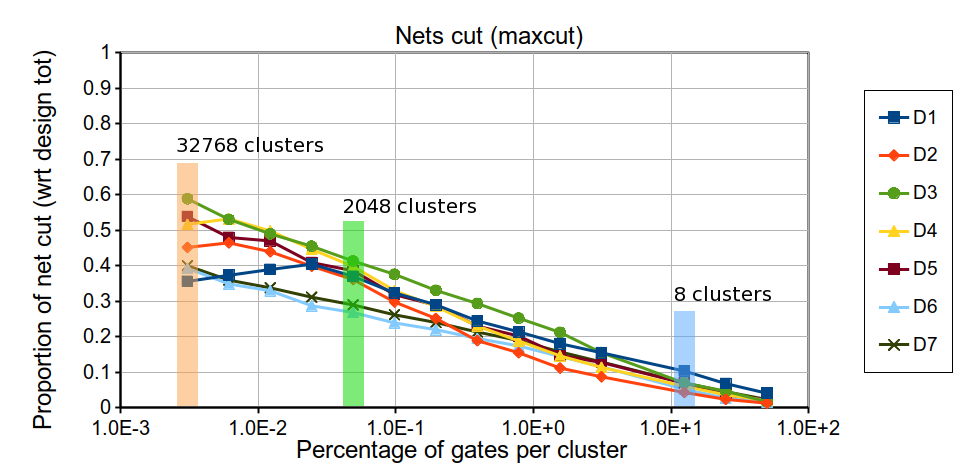
\includegraphics[height=4.5cm]{prop-netcut-wrt-design_prop-gate-per-clusters_maxcutv5_hl.png}}
%\hfill
\subfloat[]{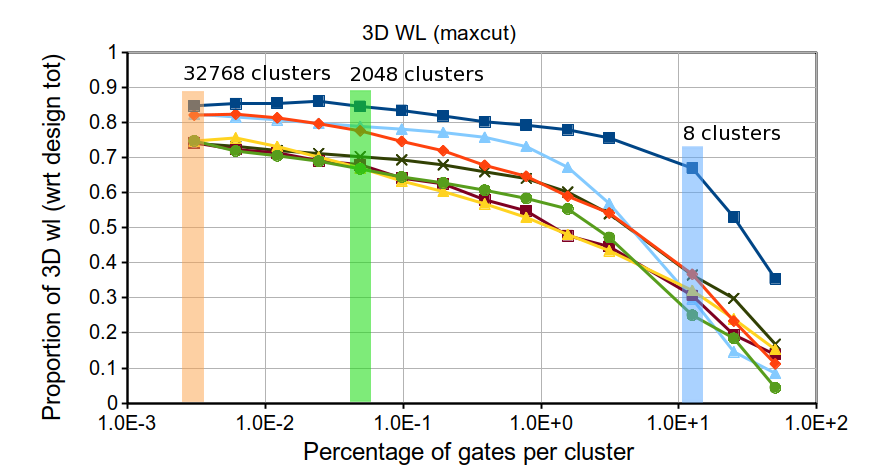
\includegraphics[height=4.5cm]{prop-3Dwl-wrt-design_prop-gate-per-clusters_maxcut_v6_hl.png}}
\caption{MAX-CUT partitioning results: Number of cut (3D) nets (a) and Ratio of total 3D wire-length (b) as function of gate-cluster size; Vertical bars corresponding to 8, 2048 and 32768 gate-clusters mark different zones in the graph}
\label{fig:3Dnets}
\end{figure*} 

\subsection{Gate-clusters}\label{sec:gate-cluster}
To generate gate-clusters we use divisive hierarchical clustering~\cite{Rokach2005} based on the geometry of the design: top-level design is first split vertically into two parts of the same size, then each part is split again, but horizontally. This process is repeated recursively -- subsequent vertical and horizontal splits -- until the targeted amount of clusters is reached. In our experiments, we consider the cluster sizes from 2 to 32768 in power-of-2 steps. The largest number of clusters (i.e. the smallest cluster size) has been picked so that the gate-count for our biggest design doesn't go below 25 gates.

\subsection{Designs data base}
For our experiments we have considered following designs: D1) an open source implementation of low-parity density parity check; D2) BoomCore: \textit{Berkeley Out-of-Order Machine}, an open source implementation of the RISC-V micro-processor; D4) MCC: a medium complexity core; D3) \& D5) respectively a crossbar and core of the OpenSparc T2 SoC;  D6) an SoC with 16 processing elements that are only locally connected (daisy chain); and D7) an SoC with 16 fully connected processing elements (each processing element is connected to all the others). Table~\ref{tab:designs} summarizes key design parameters: gate count, the total number of nets and total design wire-length after place\&route using and open-source PDK. Note that the total wire-length is normalized to design half-perimeter. 
\begin{table}
% increase table row spacing, adjust to taste
\renewcommand{\arraystretch}{1.25}
\caption{Designs data base}
\label{tab:designs}
\centering
% Some packages, such as MDW tools, offer better commands for making tables
% than the plain LaTeX2e tabular which is used here.

\begin{tabular}{||c|r|r|r||}
\hline
Design & Gates  & Nets & Wire-length\\
\hline % LDPC, HPL: 115.164, WL: 242001
D1              &  42471 &  49633 & 2101\\
\hline % BOOM, HPL: 203.968, WL: 418217
D2              & 121580 & 137171 & 2050\\
\hline % CCX, HPL: 1992.59, WL: 5698294
D3              & 185777 & 200999 & 2860\\
\hline % MCC, HPL: 242.596, WL: 1047417
D4              & 220587 & 234373 & 4318 \\
\hline % SPC, HPL: 1972.908, WL: 10479466
D5              & 289812 & 306118 & 5312\\
\hline % SoC low connectivity LDPC 4x4 serial, HPL: 477.85, WL: 6023683
D6              & 694082 & 773679 & 12606\\
\hline % SoC high-connecitivty LDPC 4x4 full, HPL: 650.176, WL: 10872106
D7              & 808199 & 883295 & 16722\\
\hline
\end{tabular}
\end{table}


\section{Results}\label{sec:res}
After graph partitioning with MAX-CUT, we analyze the number of nets that were cut (inter-cluster or 3D nets) and their length (Fig.~\ref{fig:3Dnets}). Measures are given for each level of clustering as a proportion of gates per cluster, e.g. for 100 clusters, each cluster hosts on average 1\% of all the gates in the design. Since all clusters have the same size and the distribution of the gates after placement is roughly homogeneous, it seems fair to admit that all clusters host the same amount of gates. Consequentially, an increasing number of clusters, a finer clustering grain and a reduction of number of gates per cluster all have the same meaning (going from right to left in the graphs).

Fig.~\ref{fig:3Dnets}(a) shows the proportion of nets cut by the partitioning with respect to the total amount of nets in the design. Except occasional outliers, especially for design D1 at 1.0E-2 point and as the gate-count in clusters reduces, the growth is exponential from very coarse to the finest clustering grain. Fig.~\ref{fig:3Dnets}(b) shows the proportion of 3D wire-length with respect to the total wire-length of the design. We clearly see two stages: a first exponential growth of 3D wire-length when there are few clusters, and then a second, this time linear growth leading towards a \textit{convergence region}.

An increasing number of 3D nets will translate into tighter, if not unfeasible, 3D pitch. Therefore we need to find a good compromise between the number of 3D nets and the wire-length they represent. Because of the \textit{convergence region} we can define a sweet spot when the 3D wire-length is maximized, for a minimum number of 3D nets.

Such sweet spot can be set around the 0.05\% of gates-per-cluster mark. This value corresponds to 2048 clusters and means that by cutting from 27\% to 41\% of all available nets, the total inter-cluster wire-length is in the range between 67\% and 84\% of the total wire-length, depending on the considered design. Table~\ref{tab:res} summarizes this result for all designs in our data base and this is the region where the 3D partitioning should occur. 
\begin{table}[!t]
% increase table row spacing, adjust to taste
\renewcommand{\arraystretch}{1.25}
\caption{MAX-CUT Results for Three Cluster Sizes}
\label{tab:res}
\centering
% Some packages, such as MDW tools, offer better commands for making tables
% than the plain LaTeX2e tabular which is used here.
\begin{tabular}{|c|r|r|r|r|r|r|}
\cline{2-7}
\multicolumn{1}{c|}{} & \multicolumn{3}{c|}{Percentage of nets cut} & \multicolumn{3}{c|}{Percentage of 3D WL}\\
\hline
\multicolumn{1}{|c|}{Clusters} & 8 & 2048 & 32768 & 8 & 2048 & 32768\\
\hline
Average & 7\% & 35\% & 49\% & 37\% & 73\% & 78\%\\
\hline
Std dev & 2\% & 5\% & 7\% & 13\% & 6\% & 4\%\\
\hline
\end{tabular}
\end{table}
Beyond this sweet spot total inter-cluster wire-length doesn't change much. At this level of clustering we could capture the most of inter-cluster wire-length. Refining the grain further to eventually reach single gate per cluster (i.e. monolithic 3D-integration) will not necessarily improve the system PPA.\\
Figure~\ref{fig:dits-wl-quart} show that for most designs, the nets cut by the partition have a length between 0.1\% to 10\% of the longest net cut. In particular it highlights the fact that the shortest nets are a minority, hence limiting the drop of performance when rerouting those in 3D.
% TODO Refaire la figure de distribution pour 2048 clusters
\begin{figure}[!t]
\centering
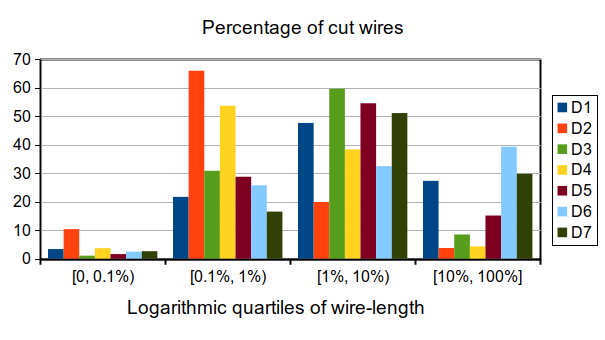
\includegraphics[width=0.9\linewidth]{netCutWL_maxcut_all_log-quart_2048.png}
\caption{Distribution of the percentage of cut wires per logarithmic quartile of their wire-length relative to the longest net, for 2048 clusters.}
\label{fig:dits-wl-quart}
\end{figure}
\section{Conclusion}\label{sec:concl}
For quite some time 3D integrated circuits are considered as potential solution to extend Moore's law. As the pitch of the 3D structures scales, allowing millions of connections per $mm^2$, the question on how, and especially at what grain, we should execute system partition when building a 3D system is becoming relevant. In this paper we have demonstrated the existence of a sweet spot for the clustering grain which maximizes the amount of inter-cluster wire-length with respect to the total system wire-length. The existence of this sweet spot tells us that in order to maximize the PPA benefits of 3D integration technology, we do not need to consider the circuit partitioning at very fine grain. In our future work, we will explore alternative clustering methods in order to further reduce the amount of short nets in the partitioning cut and further optimize partitioning decision, including multi-criteria optimization.

% use section* for acknowledgment
% \section*{Acknowledgment}

% trigger a \newpage just before the given reference
% number - used to balance the columns on the last page
% adjust value as needed - may need to be readjusted if
% the document is modified later
%\IEEEtriggeratref{3}
% The "triggered" command can be changed if desired:
%\IEEEtriggercmd{\enlargethispage{-5in}}

% references section

% can use a bibliography generated by BibTeX as a .bbl file
% BibTeX documentation can be easily obtained at:
% http://mirror.ctan.org/biblio/bibtex/contrib/doc/
% The IEEEtran BibTeX style support page is at:
% http://www.michaelshell.org/tex/ieeetran/bibtex/
\bibliographystyle{IEEEtran}
% argument is your BibTeX string definitions and bibliography database(s)
\bibliography{bibliography}
%
% <OR> manually copy in the resultant .bbl file
% set second argument of \begin to the number of references
% (used to reserve space for the reference number labels box)
%\nocite{*}


% that's all folks
\end{document}
